\section{Glyphs and Glyph-Based Visualizations}
\label{sec:relwork_glyphs}
The word \emph{glyph} is derived from the Greek word \emph{glyph$\bar{e}$} which means carving.
From the Palaeolithic age (18,000 BC) and their use of cave paintings, to the Neolithic age with petroglyphs (``stone carving''), pictures have been used to tell a story using symbols to depict particular events, objects, places, and activities (pictograms) or ideas (ideograms).
What is interesting about such pictorial approaches to story telling and communication is that there is a great intersection between visual language across vast different geological areas \cite{Eliade1991}.
This finding would indicate that symbols are key to the human conceptual system and that many of these symbolic representations are ``hard-wired'' in the brain \cite{Borgo:2013:EG,Eliade1991}.
Additionally, Egyptian hieroglyphs involve a more complex set of glyphs that pictorially represented not just ideas (ideograms), but also phonetics, and morphemes (the smallest grammatical unit of language).
The Chinese language with approximately thirteen dialects looked to pictograms and ideograms to solve communication problems between populations from different areas.
Perhaps the pictorial representations are not so clear in modern Chinese, however as illustrated in Figure \ref{fig:chinese-evolution}, this visual language has evolved from very metaphoric representations to their more abstract representations used today.
An additional feature of the Chinese language is how glyphs can be combined logically to mean something new, \eg, \emph{human being} can be combined with \emph{two} to mean \emph{humane}. 

\begin{figure}[b!]
\centering
\includegraphics[width=.7\textwidth]{images/related-work/glyphs/chinese-pictograms}
\caption{The evolution of pictorial representations adapted from \url{http://www.ocf.berkeley.edu/\~wwu/chinese/handout.html} show how pictograms have evolved into more abstract representations over time with the use of different script styles.}
\label{fig:chinese-evolution}
\end{figure}

These examples show that glyphs are not a new concept, they have been used for many thousands of years to communicate across cultures and languages.
Even now they are used in language and are prevalent in human-computer interaction via metaphoric icons representing functions. 
The definition of glyphs by Borgo \etal \cite{Borgo:2013:EG} as \emph{small visual} objects that have a \emph{meaning}, involve \emph{learning}, and are often \emph{metaphoric} bridges the definitions of glyphs in ancient Chinese writing, Hieroglyphs, and Petroglyphs to the definition of glyphs used in visualization.
The primary difference is in that instead of solely representing ideas or physical objects, glyphs for multivariate data exploration depict qualitative and/or quantitive attributes of data records using combinations of visual channels \cite{Borgo:2013:EG}.
The result should be a \emph{small, visual} object that encodes multiple dimensions (has \emph{meaning}), and requires some \emph{learning} like those glyphs shown in Figures \ref{fig:glyphs-simple-complex} A and B.
Figure \ref{fig:glyphs-simple-complex} A shows a relatively simple glyph design encompassing five dimensions: wind speed, wind direction, temperature, and location (X and Y position).
The use of metaphor, in colour for temperature, arrow orientation for direction, proximity for speed, and position for location makes this glyph intuitive to decode. 

A more complex example is given in Figure \ref{fig:glyphs-simple-complex} B) created by Duffy \etal \cite{Duffy:2014:TVCG} who encode twenty-three data attributes in a single glyph.
The overall objective of this work is the creation of a summary visualization to reduce the need for domain experts to watch and re-watch videos.
Each glyph is used to summarise one second intervals of sperm video data.
These sperm glyphs are viewed with respect to their spatial setting with each glyph representing one second of activity for each sperm cell.
Domain experts can easily get an overview of the movement of the cell and its detailed properties through one image.

Both examples have illustrated the special ability of glyph-based visualization to preserve spatial information that would not be possible using parallel coordinate plots or scatter plot matrices.
Glyph placement strategies have been covered in detail by Matt Ward's \cite{ward02} excellent survey.
This work provides a comprehensive taxonomy of different layout algorithms in 2D or 3D space: data-driven (raw); data-driven (derived); and structure-driven.

\begin{figure}[t!]
\centering
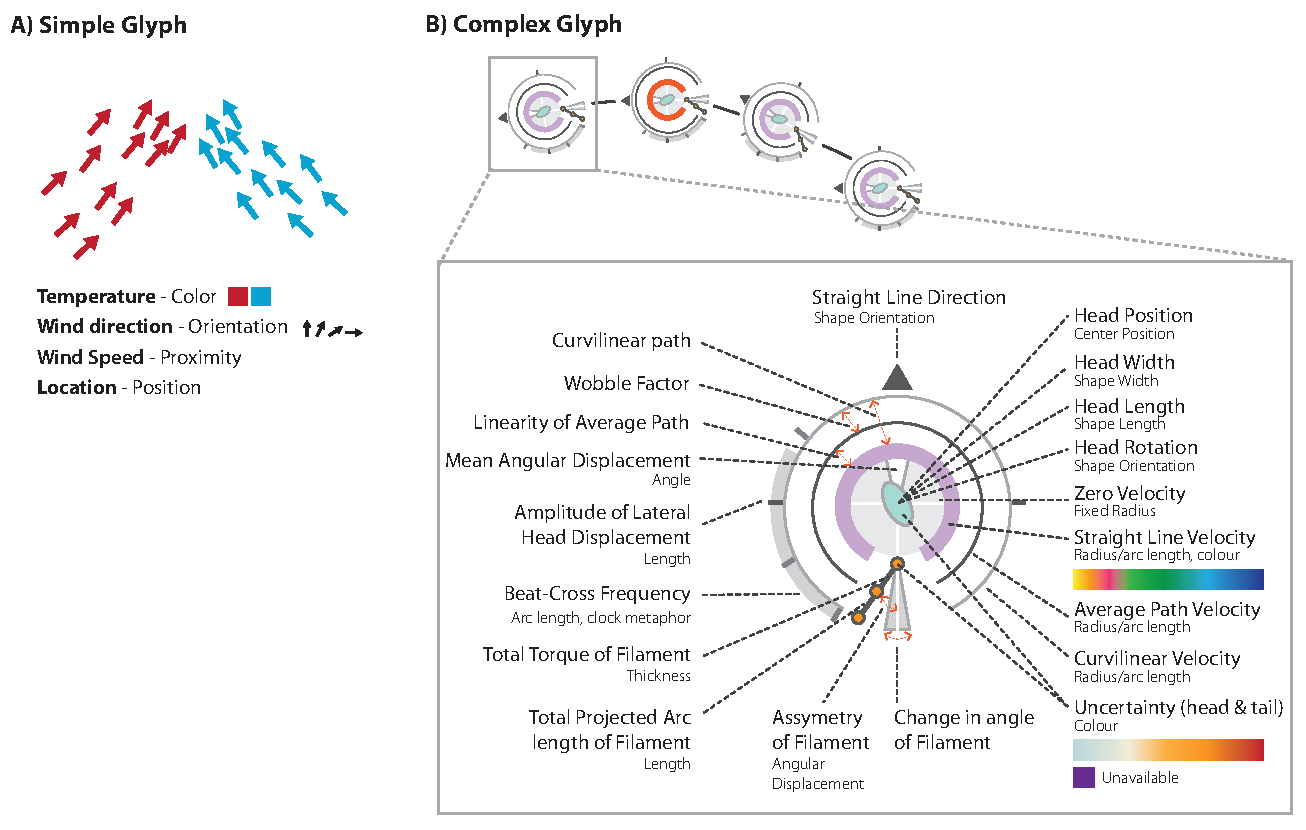
\includegraphics[width=\textwidth]{images/related-work/glyphs/glyph-simple-complex}
\caption{A) A relatively simple glyph for display of weather with five dimensions: wind speed, wind direction, temperature, and location (X and Y position). B) A more complex glyph with twenty-three dimensions by Duffy \etal depicting the attributes of sperm cells \cite{Duffy:2014:TVCG}.}
\label{fig:glyphs-simple-complex}
\end{figure}

These examples illustrate the power of glyphs in three ways: \textbf{1) multi-dimensionality} - glyphs can represent a large number of dimensions; \textbf{2) compactness} - they are able to ``compress'' a large amount of information in to a small space; and
\textbf{3) spatial preservation} - the ability to keep spatial information whilst overlaying more information.


\subsection{Glyphs and their Visual Encoding}
\label{sec:mapping-glyph-data}

Creating a glyph is often more involved than randomly assigning a data attribute to shape, colour, texture, size, or orientation.
Similar to visual signs or fonts, the design of a glyph set is in essence a visual coding scheme \cite{Borgo:2013:EG}.
Like all coding schemes, a well-designed glyph-based visualization can facilitate efficient and effective information encoding and visual communication \cite{Borgo:2013:EG}. 
A bad glyph design on the other hand may lead to ambiguity and confusion. 
Examples of good and bad coding schemes are shown in Figures \ref{fig:signs-code} A, B and C with examples based on letter discrimination and road sign design. 

Figure \ref{fig:signs-code} A shows how font choice, in essence a coding scheme, is important in the interpretation of letters. 
Using the \emph{Myriad Pro} font, many letters will not be ambiguous, such as \emph{a}, \emph{b}, and \emph{c}, however some letters will introduce ambiguity.
In the case of Illinois, the uppercase \emph{i} is not distinguishable from the lower case \emph{L}. 
While this ambiguity can be removed via context and past experience (\eg, knowing how to spell Illinois), it is a problem when previous context is not available, as is the case when learning another language. 
Change the font to \emph{Courier New}, and the ambiguity has been removed. 
Similar difficulties may arise when comparing \emph{\emph{S} and \emph{5}}, \emph{\emph{B} and \emph{8}}, \emph{\emph{A} and \emph{4}} for instance.

\begin{figure}[t!]
\centering
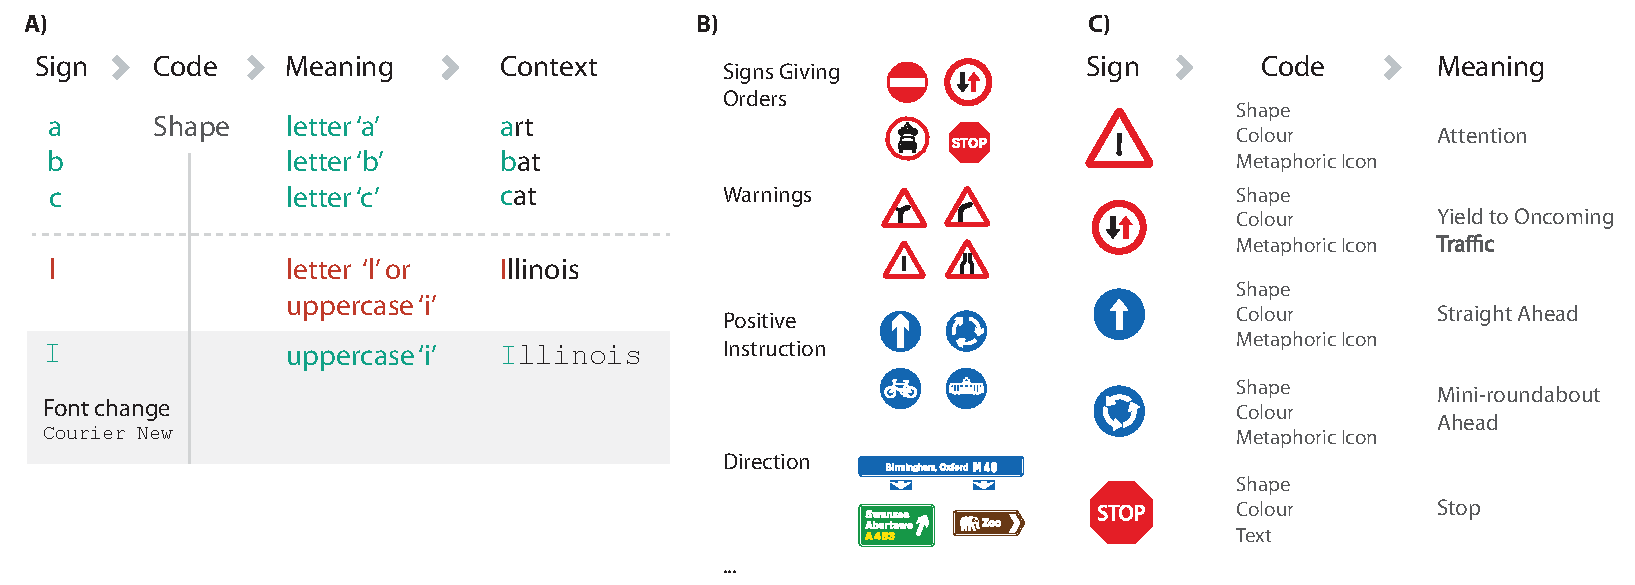
\includegraphics[width=\textwidth]{images/related-work/glyphs/signs-codes}
\caption{A) Letters are simply shapes that we assign meaning to. 
The code for creating such a shape is a particular font. 
With certain fonts, the differences between the letters is not sufficient, making it hard to find the meaning of a particular code. 
In this example, an uppercase \emph{i} can be confused with an \emph{l} (lower case \emph{L}) using the \emph{Myriad Pro} font, but is communicated more clearly using a font such as \emph{Courier New}. 
B) Road signs of the United Kingdom share some clear characteristics in different categories to make it more easy for drivers to visually select for particular pieces of information. 
C) Each sign is encoded with some information, normally pictorially to aid use by visitors from other countries and to encourage adoption as a standard across countries.}
\label{fig:signs-code}
\end{figure}

Figure \ref{fig:signs-code} B presents some classes of road signs for the United Kingdom. 
Road signs have been used for many years and have been iterated on heavily since the late 1950s \cite{kinneir1980words}. 
These iterations were made to ensure that drivers are able to find the information they are looking for (directions, warnings, \emph{etc.}) and that the most important messages are immediately visible to drivers (\eg, warnings and orders). 
If all road signs had the same general design, it would be difficult for drivers to select those signs that are important for safety from those that merely indicate the next service stop. 
If every road sign was too different from the next, drivers would have too much to remember. 
Designed by Kinneir and Calvert, U.K. road signs presented a solution in the form of categories of signs related to the type of message being communicated. 
These road signs had the additional requirement of being universally interpretable which brought challenges in ensuring visitors from other countries could recognise the signs and learn them quickly. 
This is similar to the requirement of the Chinese language to be readable by speakers of all thirteen dialects. 
This was enabled through adoption of European road signage protocols where circles indicated \emph{orders}, triangles indicated \emph{warnings}, and rectangles indicate \emph{information}. 
Colour was used carefully to add further discriminability (termed as \emph{redundant encoding}) to classes of signs, \eg, red for important warnings or orders, and blue for information signage. 
Finally, heavy use of text in previous road signs made it difficult for drivers from other countries to understand. 
Calvert introduced the use of pictograms instead of text where possible to refer to services, museums, men at work, and so on. 
This collective use of categories, shape, colour, and pictograms gave rise to the highway code, a visual language for the road in place since 1958 and a fine example of good glyph design.

Figure \ref{fig:signs-code} C illustrates a \emph{sign - code - meaning} relationship for road signs. 
In these examples and those in Figure \ref{fig:signs-code} B one may see that shape and colour play a large role in determining the type of sign while metaphor is used as much as possible to provide the internal shape. 
Metaphor is very important in the creation of signage due to the lower overhead required to remember what a sign means. 
Too many abstract shapes and colours would place a large cognitive load on anyone trying to decipher one of these codes. 
Additionally, important road signs such as \emph{stop} and \emph{no entry} are different from other signs under the \emph{giving orders} category due to their importance on the road. 
Not stopping at a junction or going up a one way street have the potential to cause great damage. 
Therefore these signs have a full red background which has a metaphoric relationship with \emph{danger}, with white text/shapes in the middle. 

\subsection{Glyph-based Visualizations}
\label{sec:glyph-examples}
From Chernoff faces \cite{chernoff1973use}, a generic glyph technique using facial attributes to represent data, to more application-specific glyphs such as the sperm glyphs by Duffy \etal \cite{Duffy:2014:TVCG}, glyphs have been used as a visualization technique across many diverse areas. 
Matt Ward provided an excellent summary of different types of glyphs in his 2002 paper \cite{ward02}.
The glyphs he identified, summarised in Figure \ref{fig:wardglyphs} included: profile glyphs (using height and colour of bars); star glyphs; Anderson/metroglyphs; stick figures; trees; auto glyphs; boxes; hedgehogs; Chernoff faces; arrows; polygons; dash tubes; weathervanes; circular profiles; colour glyphs; bugs \cite{chuah1998}; and wheels \cite{chuah1998};.

\begin{figure}[h!]
\centering
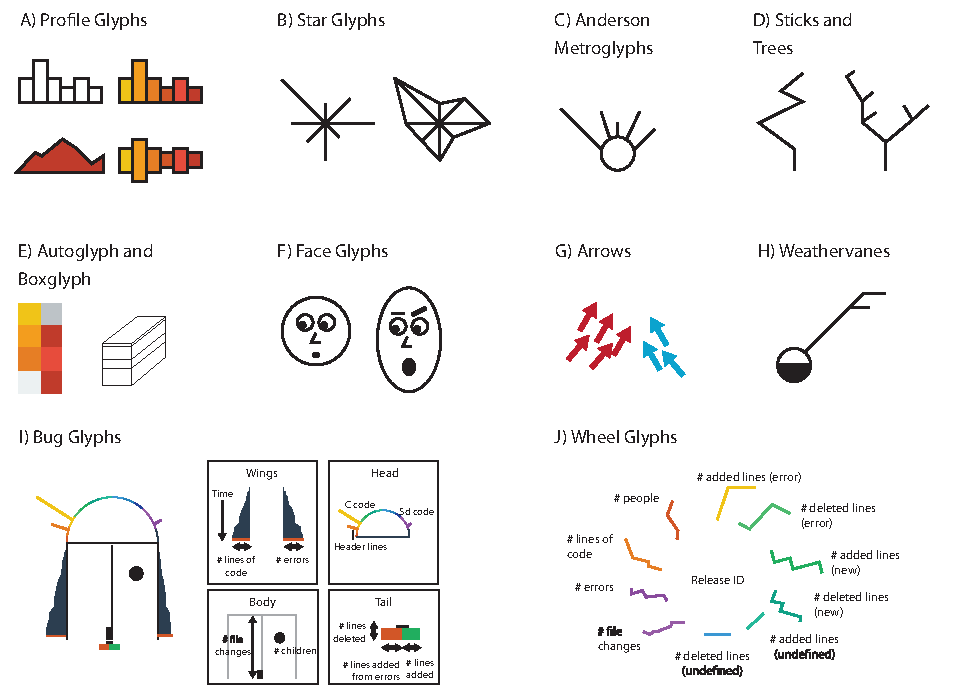
\includegraphics[width=\textwidth]{images/related-work/glyphs/glyphs_ward}
\caption{Some glyph examples from Ward \cite{ward02} with A) variations on profile glyphs; B) star glyphs; C) metroglyphs; D) stick and tree glyphs; E) Autoglyph and box glyphs: F) face glyphs (Chernoff faces); G) arrow glyphs; H) weathervanes; I) bug glyphs; and J) wheel glyphs.}
\label{fig:wardglyphs}
\end{figure}
 
Additionally, here we summarise the contribution glyphs have made in medical, event, geo-spatial, software management ,and search result visualizations.

\textbf{Medical visualization} has benefited from glyph-based visualization. 
They have been used for:
cardiac data by Ropinski and Preim \cite{ropinski08,ropinski11}, Oeltze \etal \cite{oeltze2008glyph}, and Meyer-Spradow \etal \cite{meyer2008glyph};
brain imaging, specifically (functional) magnetic resonance imaging ((f)MRI) by Tory \etal\cite{tory2001visualization}, Westin \etal \cite{westin02processing}, Zhukov and Barr \cite{zhukov2003heart}, Kindlmann \cite{kindlmann2004superquadric}, and Basu \etal \cite{basu2006rician};
and computerised tomography (CT) by Ropinski \etal \cite{ropinski2007surface}. 
A typical use case for glyphs, as identified by Ropinski and Preim, is where data from multiple sources (CT, positron emission tomography (PET) and MRI) are combined \cite{ropinski08}. 
MRI and CT data provide a detailed, high-resolution view of the anatomical structure whereas PET scans show cells that are metabolically highly active with the inclusion of glucose in the PET tracer along with a radioactive label. 
Tumour cells are typically more metabolically active than normal cells; therefore their need for energy, and therefore glucose is increased.
PET scans show these areas of activity and are pointers towards cancer sites. 
Additionally, Duffy \etal \cite{Duffy:2014:TVCG} created a glyph-based summary of videos representing sperm movement. 
For a more in-depth survey of glyph use in medical visualization, see Ropinski and Preim's recent surveys on glyph use in medical visualization \cite{ropinski08,ropinski11}.

\textbf{Event/activity visualization} is a growing area of research where glyphs are becoming a widely used technique. 
Botchen \etal \cite{botchen08ActionBasedVideo} used glyphs to create summaries of video surveillance systems. 
Such glyphs encode position of objects, size, type of action, and relation with other objects as well as statistical information about uncertainty of the analytics algorithm. 
Pearlman and Rheingans \cite{pearlman08} used glyphs to represent nodes of a computer network where different types of network events and their frequency are represented using pie charts. 
These pie charts can be nested within each other to encode changes over time. 
Legg \etal \cite{Legg:2012:CGF} used metaphoric glyphs for annotation of rugby match videos to encode information about the type of event (metaphoric pictograms), the players involved (boxes with player shirt numbers), and the team involved (colour). 

\textbf{Geo-spatial visualization} is an area where glyphs have long been used to overlay information on maps. 
In 1855, Dr. John Snow was one of the first users of glyphs in geo-spatial visualization when he used the famous map of London overlaid with cholera incidents to communicate the relation between water pumps and the location of cholera victims \cite{snow1855mode}. 
His simple glyph made use of stacked rectangles to indicate the number of incidences and position to show location. 
More recent examples include MacEachren and Brewers \cite{maceachren1998visualizing} use of colour and texture to represent the reliability of health care statistics data. 
Figure \ref{fig:glyphs-simple-complex} A shows a simple glyph visualization for weather data where the location of each arrow represents a measurement at a particular geo-spatial location. 
Weather visualizations make good use of visualization to overlay information on top of maps such as rain fall, cloud cover, temperature, and so on. 
Noodles from Sanyal \etal \cite{sanyal:2010:NTEU} use glyphs to show uncertainty in weather data. 
Ware and Plumlee \cite{Ware01072013} show how glyphs can be used to redesign weather displays.
\emph{SkyScope} by Coelho and Low\cite{coelhoskyscope} and \emph{AWE} by Spirkovska and Lodha \cite{spirkovska2002awe} use glyphs to provide pilots with weather forecasts over time including temperature, cloud cover (at different heights), precipitation, and wind direction. 
\emph{SWIM} by Lundblad \etal \cite{lundblad2009interactive} is a decision support system for use by shipping companies to plan ship routes based on weather data. 
Ships are illustrated by glyphs and their route is illustrated via a line. 
Wind speed and direction are shown via glyphs, as are ``freak'' wave events. 
Further information such as wave height, air pressure, and temperature are shown via isosurfaces. 

\textbf{Software management} is often a complicated process where one wishes to observe the productivity of developers via metrics such as lines of code added/deleted, number of errors introduced, issues closed, tests added, and so on. 
Chuah and Eick \cite{chuah1998} presented two glyph designs to encapsulate such information; bug glyphs, and wheel glyphs. 
Bug glyphs, shown in Figure \ref{fig:wardglyphs} I encode information about number of lines added, number of errors, number of file changes, and the languages used.
Wheel glyphs, shown in Figure \ref{fig:wardglyphs} J summarise dimensions such as lines of code, the number of people, errors, and file changes over time.

\textbf{Search results} are frequently rendered as text, which is sufficient for most users. However, in some domains, it would be beneficial to have more information available about the resource in the search result. 
Roberts \etal \cite{roberts2002multiform} presented the first glyph-based solution for showing \emph{Google} search results.
Chau \cite{chau2011visualizing} extended this work through the use of flower glyphs to display additional information.
Document length is shown using stem length, internal and external out links are rendered by leaf count, in links are shown by the size of the supporting ground and keywords are rendered with different petal colours.
Kachkaev \etal \cite{kachkaev2014} presented a glyph design supported by a visual analytics environment to help in navigation of survey results.
Karve \cite{Karve07} presented a glyph design for navigating search results in proteomics data. 

\textbf{Flow visualization} is a class of visualization used to show patterns in the flow of liquids, and gases where glyphs are commonly used.
For example Peng and Laramee \cite{peng2008vector} use simple arrow glyphs where flow direction is given by arrow direction, and velocity of the flow is given by colour.
An issue for such glyph-based visualizations is the visual clutter that occurs with dense collections of arrows.
Peng \etal \cite{peng2012mesh} devised a technique to reduce visual clutter through composite glyphs that show the range of velocity and direction for a cluster of arrows.
A comprehensive overview of vector field visualizations used to render such data are detailed by Peng and Laramee \cite{peng2009higher}, and more recently by Chung \etal \cite{chung2014glyph}.


More generally, tools such as \emph{GlyphMaker} from Ribarsky \etal \cite{ribarsky94} enable users to map data variables to different visual channels of a glyph (position, colour, shape, size, and transparency).
Additionally, for scientific (three dimensional) data, Kraus and Ertl \cite{Kraust01} proposed a similar type of tool.
%Due to the importance of metaphor in glyphs so as to enable memorability, it is difficult to have very glyphs that work equally well across discipline such as medicine, physics, biology, and business
